\documentclass{article}

% if you need to pass options to natbib, use, e.g.:
%     \PassOptionsToPackage{numbers, compress}{natbib}
% before loading neurips_2018

% ready for submission
% \usepackage{neurips_2018}

% to compile a preprint version, e.g., for submission to arXiv, add add the
% [preprint] option:
    \usepackage[preprint]{neurips_2018}

% to compile a camera-ready version, add the [final] option, e.g.:
     % \usepackage[final]{neurips_2018}

% to avoid loading the natbib package, add option nonatbib:
    % \usepackage[nonatbib]{neurips_2018}

\usepackage[utf8]{inputenc} % allow utf-8 input
\usepackage[T1]{fontenc}    % use 8-bit T1 fonts
\usepackage{graphicx}
\usepackage[font=small,labelsep=period]{caption}
\usepackage{subfigure}
\usepackage{hyperref}       % hyperlinks
\usepackage{url}            % simple URL typesetting
\usepackage{booktabs}       % professional-quality tables
\usepackage{amsfonts}       % blackboard math symbols
\usepackage{nicefrac}       % compact symbols for 1/2, etc.
\usepackage{microtype}      % microtypography
\usepackage{pifont}
\usepackage{enumerate}
\usepackage{amsmath}
\usepackage{enumitem}
\setlist[enumerate,1]{label=(\arabic*),font=\textup,
leftmargin=7mm,labelsep=1.5mm,topsep=0mm,itemsep=-0.8mm}
\usepackage{algorithm}
\usepackage{algpseudocode}
\usepackage{booktabs}
\renewcommand{\algorithmicrequire}{\textbf{Input:}}  % Use Input in the format of Algorithm
\renewcommand{\algorithmicensure}{\textbf{Output:}} % Use Output in the format of Algorithm
\newcommand{\topcaption}{\setlength{\abovecaptionskip}{0pt} \setlength{\belowcaptionskip}{10pt} \caption}


\title{Detecting Adversarial Examples via Undercover Attack}

% The \author macro works with any number of authors. There are two commands
% used to separate the names and addresses of multiple authors: \And and \AND.
%
% Using \And between authors leaves it to LaTeX to determine where to break the
% lines. Using \AND forces a line break at that point. So, if LaTeX puts 3 of 4
% authors names on the first line, and the last on the second line, try using
% \AND instead of \And before the third author name.

\author{%
  Qifei Zhou \\ %\thanks{}
  School of Software and Microelectronics\\
  Peking University\\
  Beijing 100871, China \\
  \texttt{qifeizhou@pku.edu.cn} \\
  % examples of more authors
  \And
  Weiping Li \\
  School of Software and Microelectronics\\
  Peking University\\
  Beijing 100871, China \\
  \texttt{wpli@ss.pku.edu.cn} \\
  \AND
  Tong Mo \\
  School of Software and Microelectronics\\
  Peking University\\
  Beijing 100871, China \\
  \texttt{motong@ss.pku.edu.cn} \\
  \And
  Yue Wu \\
  Logistics Engineering \\
  University of Science and Technology Beijing \\
  Beijing 100083, China \\
  \texttt{869216739@qq.com} \\
  % \And
  % Coauthor \\
  % Affiliation \\
  % Address \\
  % \texttt{email} \\
}

\begin{document}
% \nipsfinalcopy is no longer used

\maketitle

\begin{abstract}

\end{abstract}

\section{Introduction}
 
Both Deep nerual networks (DNNS) and Recurrent nerual networks (RNNS) are vulneralbe to adverisarial examples \cite{Szegedy2013Intriguing,Goodfellow2014Explaining,Papernot2016Transferability,papernot2016crafting}, imperceptible modifications to the original inputs of a classifier can cause the model to produce incorrect outputs. This problem is especially important in safety-critical applications such as self-driving cars. To illustrate how adversarial samples make a system based on DNNs vulnerable, consider the following 
images \ref{car}:

\begin{figure}[h]
  \centerline{
    \subfigure[prohibition sign]{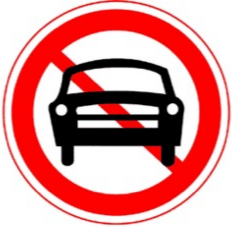
\includegraphics[scale=0.3]{car.png}}
    \subfigure[fire sign]{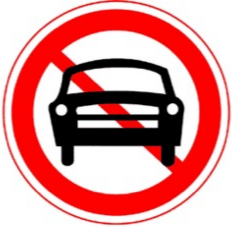
\includegraphics[scale=0.3]{car.png}}
  }
  \caption{(a) is the original image of a prohibition sign and (b) is the adversary of (a)}
  \label{car}
\end{figure}

To humans, these two images look the same: we identify each of them as a prohibition sign. The image on the left is indeed an ordinary image of a prohibition sign. We produced the image on the right by adding a very small perturbation that forces a particular DNN to classify it as a fire sign. The work or Kurakin et al. \cite{Kurakin2016Adversarial} showed that these transformations are effective in the physical world. Here, someone with ulterior motives can make self-driving cars behave dangerously taking advantage of the vulnerability of DNNs. 

There are numerous methods have been proposed to fool the model in image classification tasks, such as L-BFGS \cite{Szegedy2013Intriguing}, FGSM \cite{Goodfellow2014Explaining}, BIM \cite{Kurakin2016Adversarial}, JSMA \cite{papernot2016the} and C\&W \cite{Carlini2016Towards}. This problem has aroused great concern in the academic world. Many researchers has being trying to explain adversarial examples and find new ways to defend aganist these attack methods. There are numerous defense techniques including image compression or filtering \cite{das2017keeping,xu2018feature}, defensive distillation \cite{papernot2016distillation} and many defenses summarized as Gradient masking \cite{Papernot2016Transferability} or Obfuscated Gradients \cite{athalye2018obfuscated}. Unfortunately, none of these defenses is yet completely satisfactory, they can generally be evaded by stronger attacks wholly or partially. The most popular defense in current research papers is probably adversarial training proposed by Goodfellow et al. \cite{Goodfellow2014Explaining} which also helps us a lot in \emph{Undercover Attack}.

Due to the challenge of defenses, many recent work has turned to detect adversarial examples. Xu et al. used feature squeezing to detect, while such detectors may work well against certain attacks, detectors in this category have been shown to fail in the white box case, where the attacker is aware of the detector \cite{He2017Adversarial}. Feinman et al. \cite{feinman2017detecting} showed that Kernel Density estimates and Bayesian Uncertainty estimates can detect points lie in low-confidence regions of the input space. Pang et al. \cite{pang2018towards} proposed a new loss function named Reverse Cross-entropy which can improve the performance of KD and BU. Howerver, KD and BU have been debeated by C\&W in \cite{carlini2017adversarial} who showed that incorporating kernel density into the objective function makes detection substantially more difficult. Ma et al. \cite{ma2018characterizing} proposed Local Intrinsic Dimensionality which is claimed robust to C\&W and achieves quite execellent performance on various attacks both in black-box and white-box. KD, BU and LID all rely on knowledge of the attack mechanism. They need to train on adversarial examples generated by these attack methods which can't cope with new attacks. Inspired by the use of biometric and cryptograpic signatures, Dathathri et al. \cite{dathathri2018detecting} proposed NeuralFingerprinting (NeuralFP). They trained the model with NeuralFP which achieved near perfect AUC-scores aganist black-box attacks. While, just like in cryptography, the model can't guarantee its effectiveness if the NeuralFP is exposed to us.

Most of these attacks and defenses can't directly be used to craft adversarial sequences misleading RNNS in the scenario of Natural language processing (NLP). Papernot et al. \cite{papernot2016crafting} adapted Jacobian based algrothim to craft adversarial sequences. He made some changes of JSMA in computer vision, because the set of legitimate word embedding is finite. Rosenberg et al. proposed to use Adversarial Training, Adversarial Signatures, Rnn Ensemble and Defense SeqGAN to make an RNN classifier robust aganist adversarial examples. Adversarial Training get the best detection performace with 89.39\% Recall and 92.10\% Accuracy.

We have been working hard to study and explain the vulnerability of normal samples all the times. However, we didn't realize that adversarial samples are more vulnerable than normal ones, especially in Computer Vision. It may be not easy to sucessfully attack a benign example, and we even can't find any adversarial examples within the $\epsilon$ norm ball of the benign example as long as $\epsilon$ is small enough. Nevertheless, there must be some small modifications which can attack an adversarial example sucessfully. Because the adversarial example is generated from a benign example, we can find at least one way which is rolling back to the benign one. This is a successful attack for the adversarial example (In our paper, a successful attack is an attack which changes the model's prediction, not necessary the true lable. Especially for an adversarial input, its prediction is not exactly the true class). In fact, our experiments show that adversarial examples is far more vulnerable than normal examples. We design \emph{Undercover Attack} to detect adversarial examples based on this property. Althogh, the characteristics may be completely different in NLP, \emph{Undercover Attack} can also get perfect 100\% AUC-socres with no adversarial training or anything else. There are some intriging things between CV and NLP when adapted \emph{Undercover Attack} to them, we will discuss it in detail in Section 3.

Our key contributions are:

\begin{itemize}

  \item We propose \emph{Undercover Attack} to detect adversarial examples. \emph{Undercover Attack} is a novel idea which defends by attacks. We discuss how \emph{Undercover Attack} can distinguish adversarial samples in Computer Vision and Natural language processing seperately. Experients show that it is easier to attack adversarial samples successfully than normal samples.

  \item \emph{Undercover Attack} does not rely on knowledge of the attack mechanism. Our framework does not require additional detectors, networks or parameters. And we emperically show that the performance of \emph{Undercover Attack} is robust to unknown attack methods.

  \item  To the best of our knowledge, we are the first to introduce a adversarial detection mechanism which can be both adapted to attacks on images and sequences with excellent performance. When faced with unknown and white-box attacks, \emph{Undercover Attack} achieves state-of-the-art AUC-scores with an average performace of 97\% on various attacks on both MNIST and CIFAR10 datasets. The most exciting thing is that \emph{Undercover Attack} achieves perfect 100\% AUC-scores with RNNS on the movie review dataset IMDB.

  % In the same difficult scenario: unknown attack, 

  % \item Our study reveals that even very simple attack mechanism, like FGSM can attack adversarial samples with high success rate.  We train our model on the FGSM attack strategy, after training, our model is robust to FGSM attack on normal samples. However, if we generate adversarial examples through stronger attack mechanisms and then utilize FGSM to attack these adversarial examples, we can always succeed.

\end{itemize}

\section{Adversarial Attacks}

The typical goal of an adversary is to generate a sample which looks like a normal example, but it is misclassified by the target model. It means to modify few pixels with small perturbations of inputs in CV and change few words of inputs in NLP. This amounts to making minor changes to the inputs, causes the target model to misclassify the sample, but remains correctly classify by human. A significant number of adversarial attacks satisfying this goal have been proposed in recent years. This allows us a wide range of attacks to choose from in our investigation. Here, we introduce some of the most well-known attacks.

\subsection{Fast Gradient Sign Method (FGSM)}

Goodfellow et al. hypothesized that adversarial examples can be found using only a linear approximation of the target model \cite{Goodfellow2014Explaining}. They introduced the Fast Gradient Sign Method for efficiently crafting adversarial examples. 

\begin{equation}
  X^{adv}=X+\epsilon sign(\bigtriangledown_X J(\theta,X,y_{true}))
\end{equation}

FGSM works by linearizing loss function in $L_\infty$ neighbourhood of a clean image. $\epsilon$ is a parameter determines the perturbation size in the direction of the gradient, $\theta$ represents the parameters of the model, $y_true$ is the correct label of X.

\subsection{Basic Iterative Method (BIM, I-FGSM)}

Kurakin et al. apply FGSM multiple times with small step size \cite{Kurakin2016Adversarial} which called Basic Iterative Method or Iterative FGSM. $\alpha$ is the perturbation size in each iteration, $Clip_{X,\epsilon}(\cdot)$ performs per-pixel clipping of the image X, so $X^{adv}$ will be in $L_\infty$ $\epsilon$-neighbourbood of the clean image X.

\begin{equation}
  X_0^{adv}=X, \hspace{0.5cm} X_{n+1}^{adv}=Clip_{X,\epsilon}\{X_n^{adv}+\alpha sign(\bigtriangledown_X J(\theta,X_n^{adv},y_{true}))\}
\end{equation}

\subsection{Jacobian-based Saliency Map Attack (JSMA)}

Papernot et al. \cite{papernot2016the} introduced Jacobian-based Saliency Map Attack for targeted misclassification. The above two methods (FGSM, BIM) modifies each pixel with small $\epsilon$-ball perturbation, JSMA works by modifying a limited number of input pixels with relatively large perturbations instead. JSMA iteratively perturbs pixels that have high adversarial saliency scores. Euqation \ref{jsma} explains how to calculate adversarial saliency scores. To achieve a target class t, $F_t(X)$ must be increased while the probabilities of all other classes $\Sigma_{j\neq t} \frac{\partial F_j(X)}{\partial X_i}$ decrease.

\begin{equation}
  S(X,t)[i]=
  \left\{
  \begin{array}{rcl}
    0, \mbox{ if } \frac{\partial F_t(X)}{\partial X_i}<0 \mbox{ or } \Sigma_{j\neq t} \frac{\partial F_j(X)}{\partial X_i}>0 \hfill \\
    (\frac{\partial F_t(X)}{\partial X_i})|\Sigma_{j\neq t} \frac{\partial F_j(X)}{\partial X_i}|, \mbox{ otherwise}          \hfill
  \end{array}
  \right.
  \label{jsma}
\end{equation}

\subsection{Carlini and Wagner Attack (C\&W)}

N.Carlini and D.Wagner introduced a optimization attack framework \cite{carlini2017adversarial} that passed a range of attacks. They designed a loss function that has smaller values on adversarial samples and higher on benign samples. This results in three kind of attacks: an $L_\infty$ attack, an $L_0$ attack, and an $L_2$ attack. They achieved the strongest $L_2$ attack which we will consider in this paper with the following loss function:

\begin{equation}
  \mbox{minimize } ||\frac{1}{2}(tanh(w)+1)-x||_2^2+c\cdot f(\frac{1}{2}(tanh(w)+1))
\end{equation}

$f(\cdot)$ is based on the best objective function found earlier, which is defined as:

\begin{equation}
  f(x^{'})=max(max\{Z(x^{'})_i:i\neq t\}-Z(x^{'})_t,-k)
\end{equation}

Here, k is a parameter control the misclassification confidence, we can find adversarial examples with high confidence by adjusting k.

\subsection{Jacobian-based Attack On RNNs}

Papernot et al. \cite{papernot2016crafting} showed that the algrothims introduced previously to craft adversarial instances misclassified by feed-forward neural networks can be adapted to recurrent neural works. However, these methods can't be adapted to natural language processing tasks directly due to the finite set of word embeddings. That's to say that we can't modify the word embeddings casually, because we may not find a real word corresponding to the modified word embeddings. They followed a heuristic procedure to solve the problem. They iteratively find a word $\vec{z}$ in words set that the sign of the difference between the embeddings of $\vec{z}$ and the original input word is closet to $sgn(J_f(\vec{x})[i,f(\vec{x})])$. Eventually, they achieved an error rate of 100\% by changing 9.18 words in 71.06-word-long sentences on average. Later on, we will discuss our method based on Jacobian which perform better in the next section.



\section{Undercover Attack}

\section{Experiments}


\section{Conclusion}














\subsubsection*{Acknowledgments}

We would like to thank Zhilong Hong and Haochen Li for helpful discussions and their useful advice on the topic. %We also thank xxx for providing research funding support. 

\small
\bibliographystyle{plain}
\bibliography{ref}
\end{document}